\documentclass[11pt]{article}
\usepackage[textwidth=18.0cm, textheight=23.0cm, top=2.0cm]{geometry}
\usepackage{pst-all}
\usepackage{amssymb}
\usepackage{tikz}
\usepackage{underscore}\begin{document}
\pagestyle{empty}


ClassName: \underline{\textbf{Class_08.2bp-29}}
\par
BinSize: \underline{\textbf{100 × 100}}
\par
ReduceSize: \underline{\textbf{100 × 100}}
\par
TypeNum: \underline{\textbf{60}}
\par
Num: \underline{\textbf{60}}
\par
OutS: \underline{\textbf{180000}}
\par
InS: \underline{\textbf{149844}}
\par
Rate: \underline{\textbf{0.832}}
\par
UB: \underline{\textbf{18}}
\par
LB0: \underline{\textbf{18}}
\par
LB: \underline{\textbf{18}}
\par
LBWithCut: \underline{\textbf{18}}
\par
NodeCut: \underline{\textbf{0}}
\par
ExtendedNodeCnt: \underline{\textbf{1}}
\par
GenNodeCnt: \underline{\textbf{1}}
\par
PrimalNode: \underline{\textbf{0}}
\par
ColumnCount: \underline{\textbf{18}}
\par
TotalCutCount: \underline{\textbf{0}}
\par
RootCutCount: \underline{\textbf{0}}
\par
LPSolverCnt: \underline{\textbf{1}}
\par
PricingSolverCnt: \underline{\textbf{0}}
\par
BranchAndBoundNum: \underline{\textbf{1}}
\par
isOpt: \underline{\textbf{true}}
\par
TimeOnInitSolution: \underline{\textbf{600.000 s}}
\par
TimeOnPrimal: \underline{\textbf{0.000 s}}
\par
TimeOnPricing: \underline{\textbf{0.000 s}}
\par
TimeOnRmp: \underline{\textbf{0.063 s}}
\par
TotalTime: \underline{\textbf{600.313 s}}
\par
\newpage


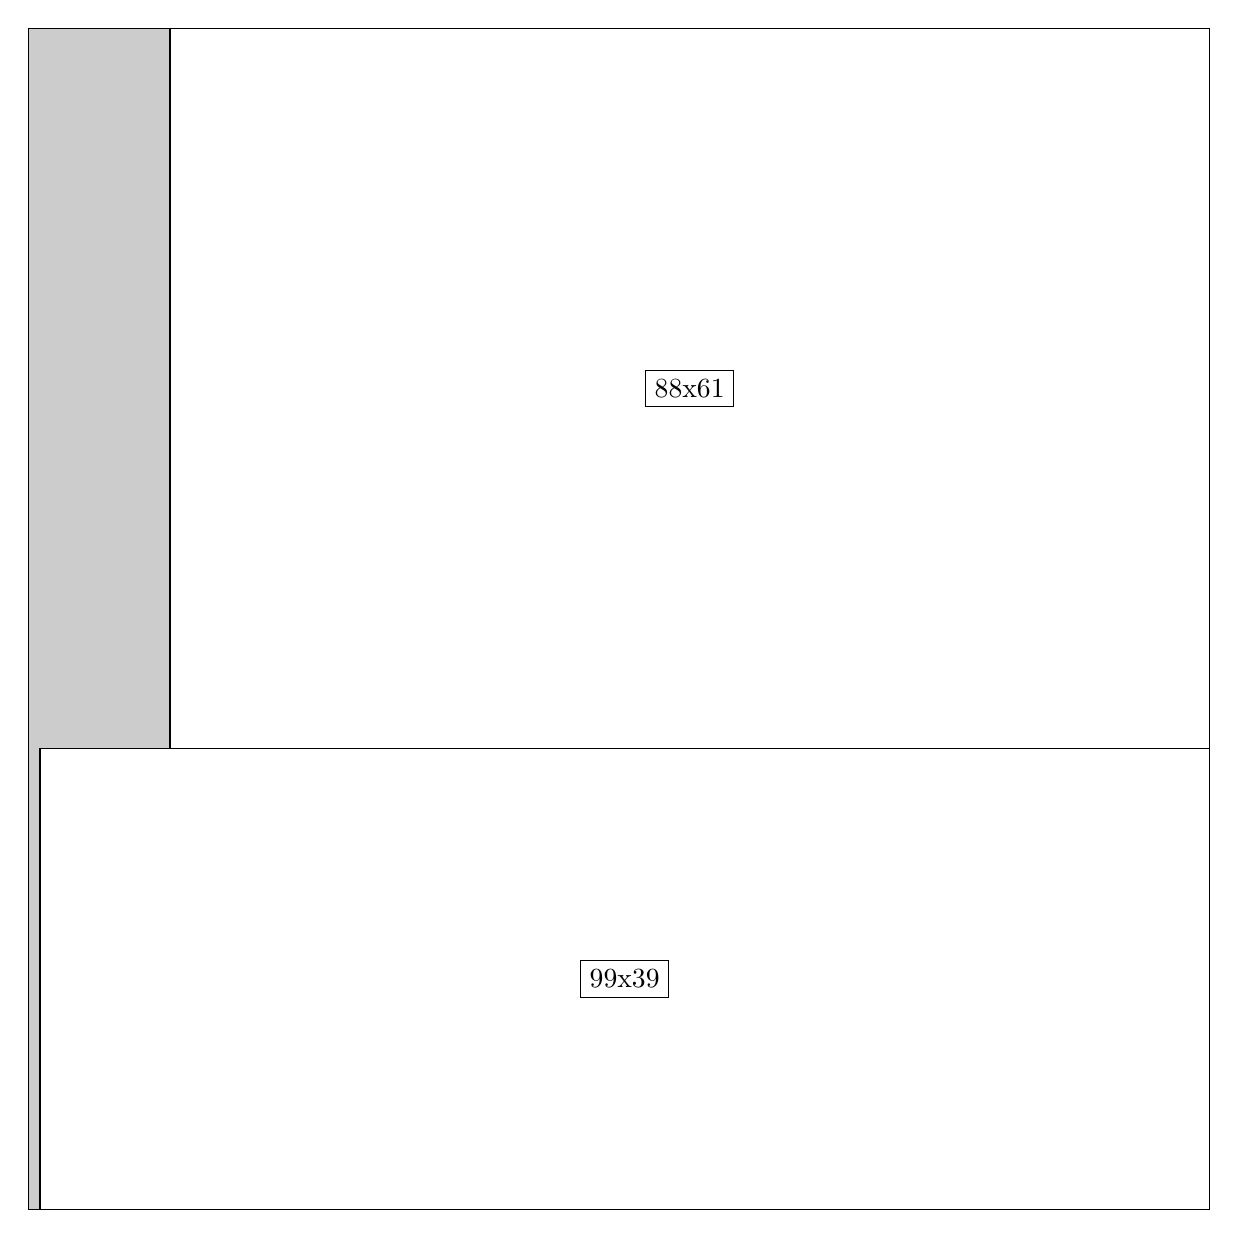
\begin{tikzpicture}[shorten >=1pt,scale=1.0,every node/.style={scale=1.0},->]
\tikzstyle{vertex}=[circle,fill=black!25,minimum size=14pt,inner sep=0pt]
\filldraw[fill=gray!40!white, draw=black] (0,0) rectangle (15.0,15.0);
\foreach \name/\x/\y/\w/\h in {99x39/0.15/0.0/14.85/5.85,88x61/1.7999999999999998/5.85/13.2/9.15}
\filldraw[fill=white!40!white, draw=black] (\x,\y) rectangle node[draw] (\name) {\name} ++(\w,\h);
\end{tikzpicture}


w =99 , h =39 , x =1 , y =0 , v =3861
\par
w =88 , h =61 , x =12 , y =39 , v =5368
\par
\newpage


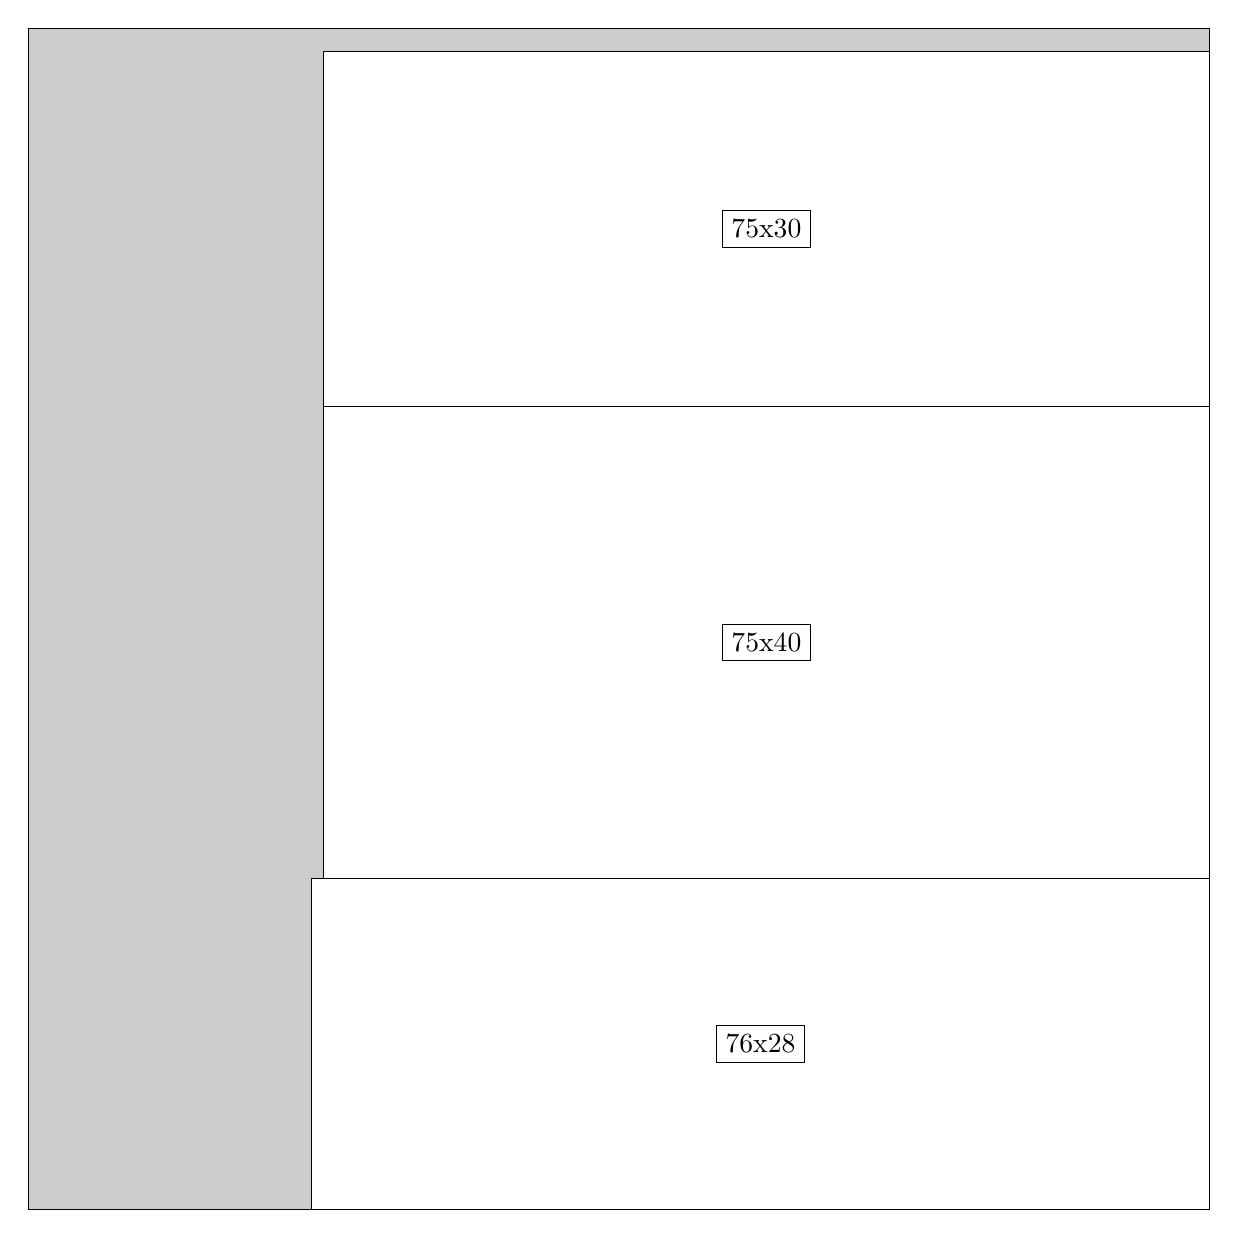
\begin{tikzpicture}[shorten >=1pt,scale=1.0,every node/.style={scale=1.0},->]
\tikzstyle{vertex}=[circle,fill=black!25,minimum size=14pt,inner sep=0pt]
\filldraw[fill=gray!40!white, draw=black] (0,0) rectangle (15.0,15.0);
\foreach \name/\x/\y/\w/\h in {76x28/3.5999999999999996/0.0/11.4/4.2,75x40/3.75/4.2/11.25/6.0,75x30/3.75/10.2/11.25/4.5}
\filldraw[fill=white!40!white, draw=black] (\x,\y) rectangle node[draw] (\name) {\name} ++(\w,\h);
\end{tikzpicture}


w =76 , h =28 , x =24 , y =0 , v =2128
\par
w =75 , h =40 , x =25 , y =28 , v =3000
\par
w =75 , h =30 , x =25 , y =68 , v =2250
\par
\newpage


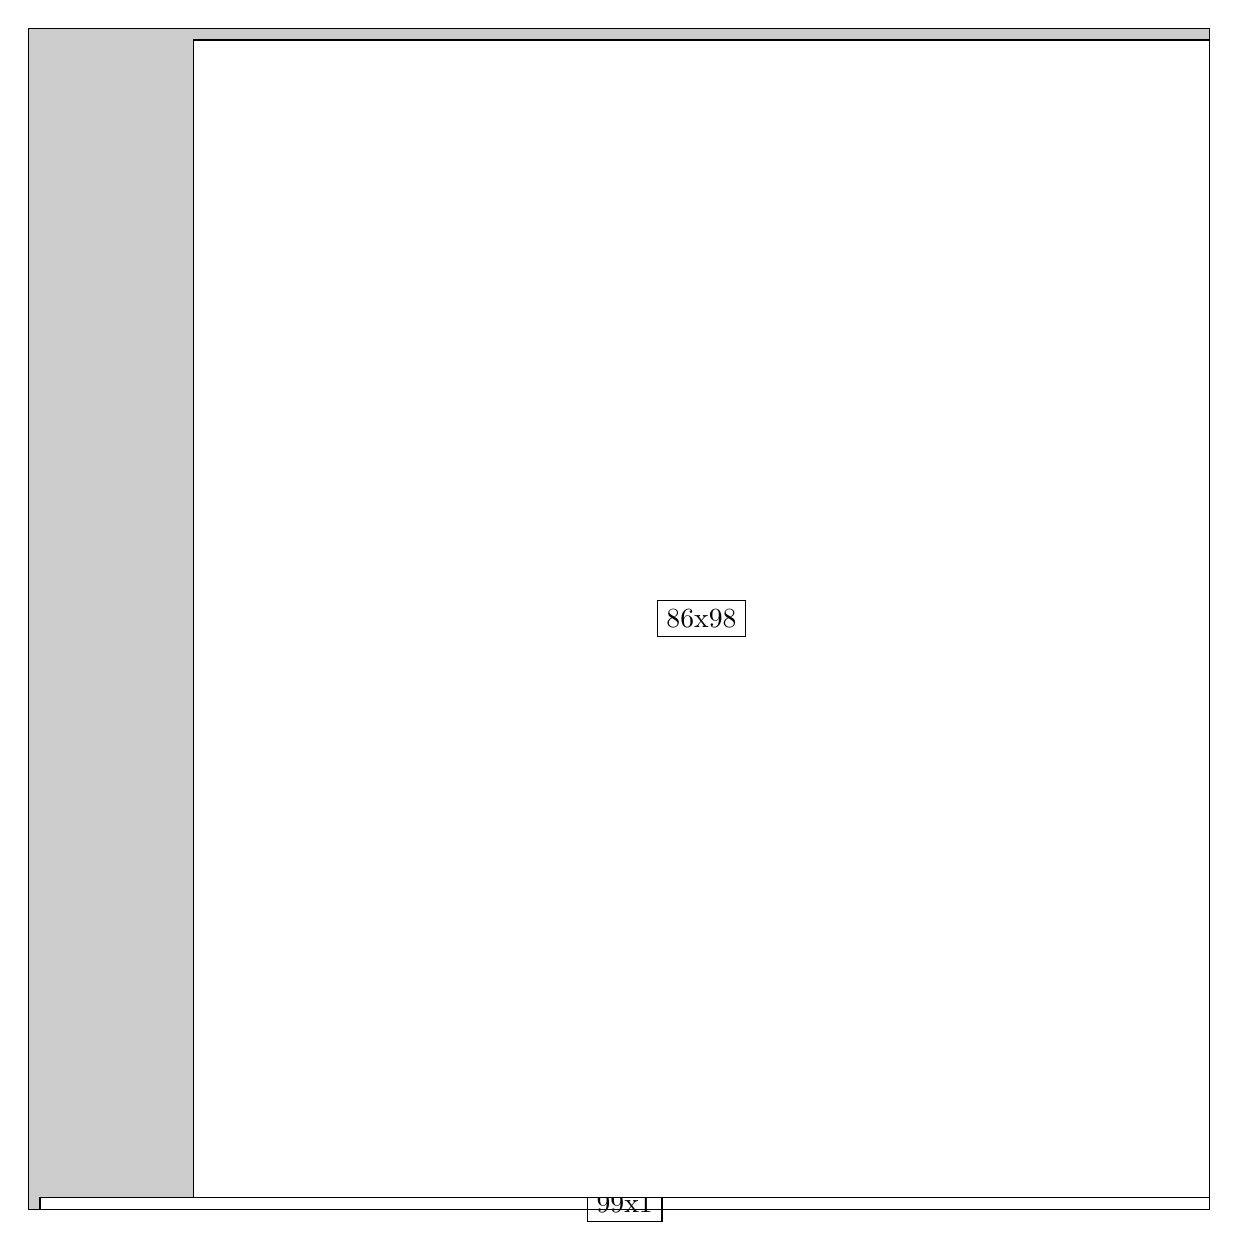
\begin{tikzpicture}[shorten >=1pt,scale=1.0,every node/.style={scale=1.0},->]
\tikzstyle{vertex}=[circle,fill=black!25,minimum size=14pt,inner sep=0pt]
\filldraw[fill=gray!40!white, draw=black] (0,0) rectangle (15.0,15.0);
\foreach \name/\x/\y/\w/\h in {99x1/0.15/0.0/14.85/0.15,86x98/2.1/0.15/12.9/14.7}
\filldraw[fill=white!40!white, draw=black] (\x,\y) rectangle node[draw] (\name) {\name} ++(\w,\h);
\end{tikzpicture}


w =99 , h =1 , x =1 , y =0 , v =99
\par
w =86 , h =98 , x =14 , y =1 , v =8428
\par
\newpage


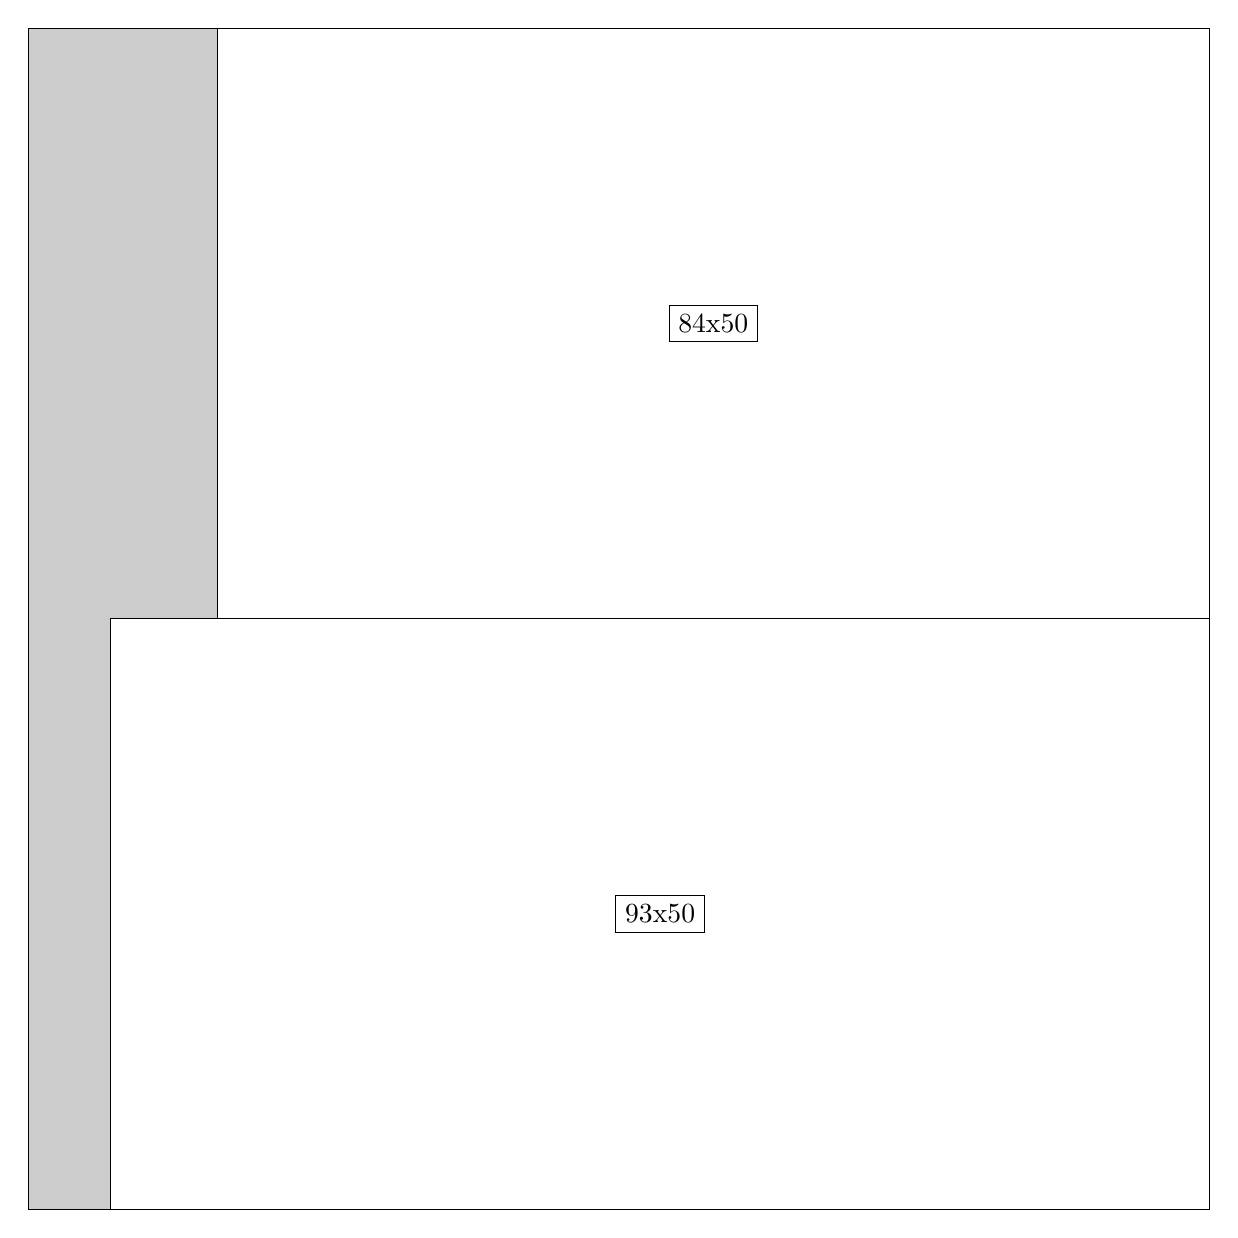
\begin{tikzpicture}[shorten >=1pt,scale=1.0,every node/.style={scale=1.0},->]
\tikzstyle{vertex}=[circle,fill=black!25,minimum size=14pt,inner sep=0pt]
\filldraw[fill=gray!40!white, draw=black] (0,0) rectangle (15.0,15.0);
\foreach \name/\x/\y/\w/\h in {93x50/1.05/0.0/13.95/7.5,84x50/2.4/7.5/12.6/7.5}
\filldraw[fill=white!40!white, draw=black] (\x,\y) rectangle node[draw] (\name) {\name} ++(\w,\h);
\end{tikzpicture}


w =93 , h =50 , x =7 , y =0 , v =4650
\par
w =84 , h =50 , x =16 , y =50 , v =4200
\par
\newpage


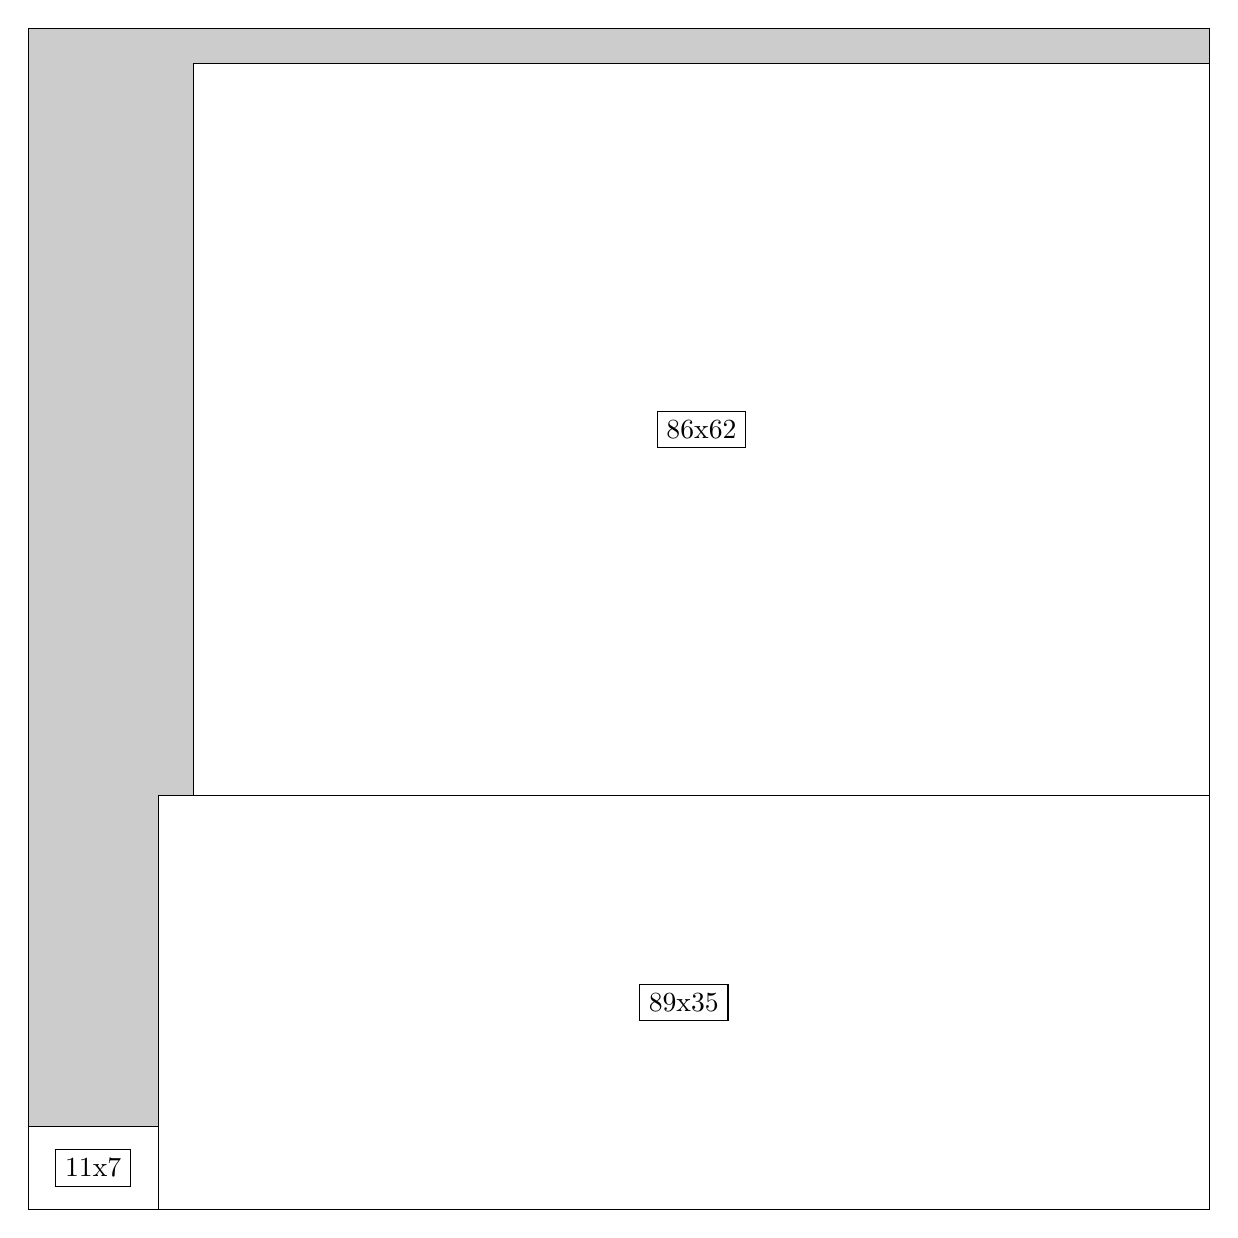
\begin{tikzpicture}[shorten >=1pt,scale=1.0,every node/.style={scale=1.0},->]
\tikzstyle{vertex}=[circle,fill=black!25,minimum size=14pt,inner sep=0pt]
\filldraw[fill=gray!40!white, draw=black] (0,0) rectangle (15.0,15.0);
\foreach \name/\x/\y/\w/\h in {89x35/1.65/0.0/13.35/5.25,11x7/0.0/0.0/1.65/1.05,86x62/2.1/5.25/12.9/9.299999999999999}
\filldraw[fill=white!40!white, draw=black] (\x,\y) rectangle node[draw] (\name) {\name} ++(\w,\h);
\end{tikzpicture}


w =89 , h =35 , x =11 , y =0 , v =3115
\par
w =11 , h =7 , x =0 , y =0 , v =77
\par
w =86 , h =62 , x =14 , y =35 , v =5332
\par
\newpage


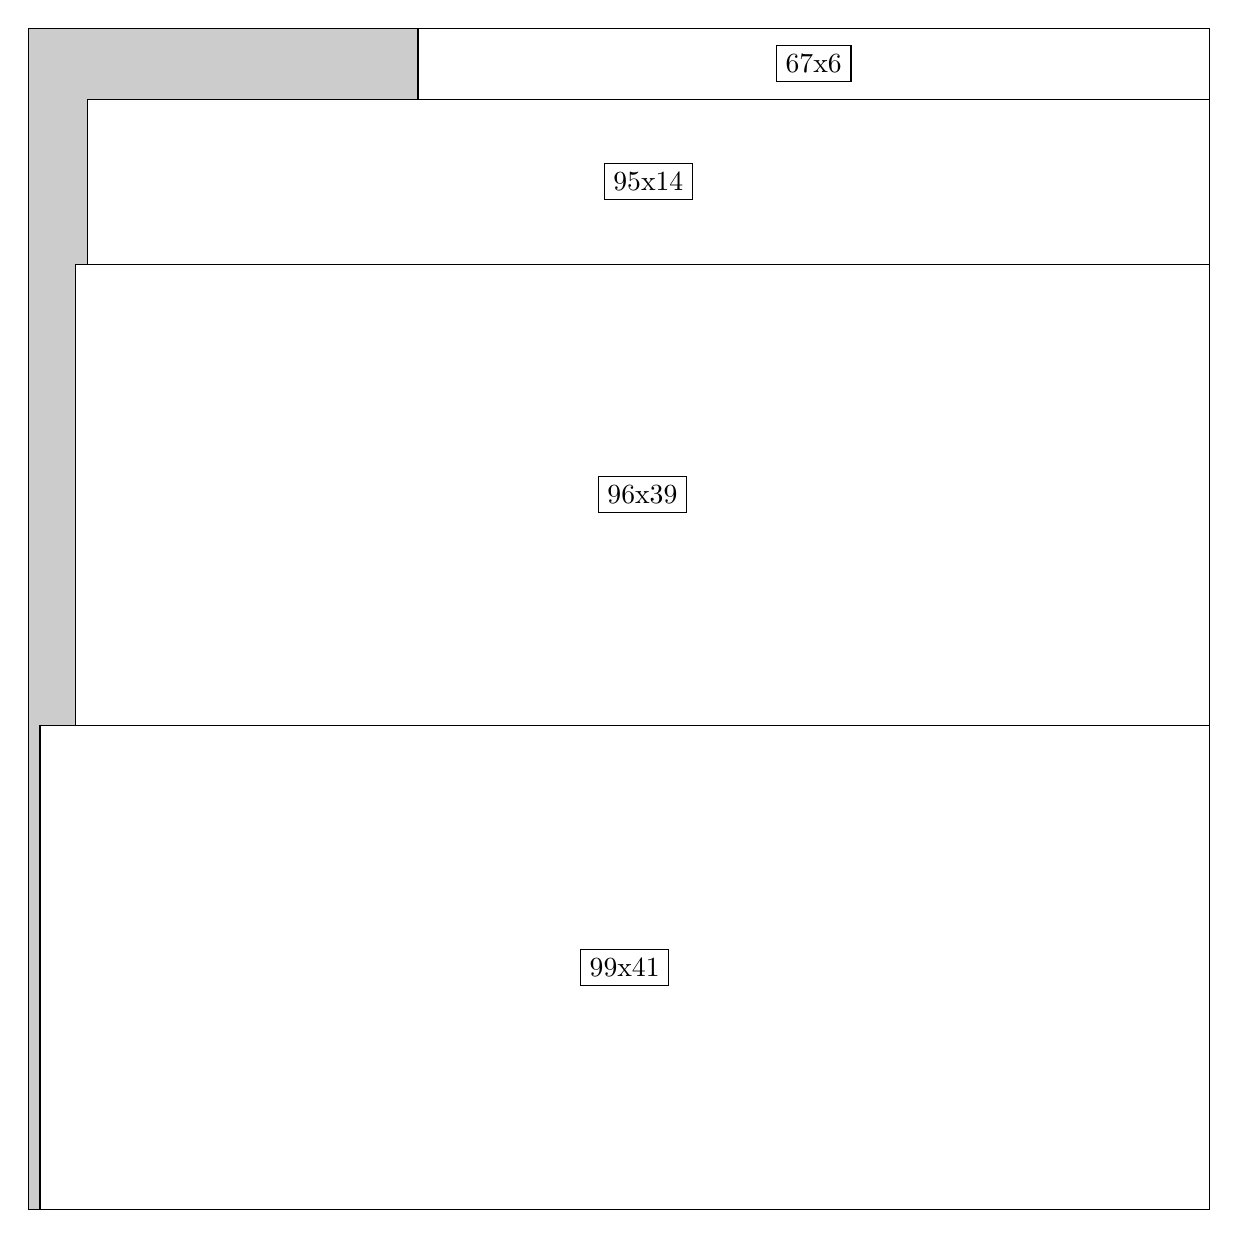
\begin{tikzpicture}[shorten >=1pt,scale=1.0,every node/.style={scale=1.0},->]
\tikzstyle{vertex}=[circle,fill=black!25,minimum size=14pt,inner sep=0pt]
\filldraw[fill=gray!40!white, draw=black] (0,0) rectangle (15.0,15.0);
\foreach \name/\x/\y/\w/\h in {99x41/0.15/0.0/14.85/6.1499999999999995,96x39/0.6/6.1499999999999995/14.399999999999999/5.85,95x14/0.75/12.0/14.25/2.1,67x6/4.95/14.1/10.049999999999999/0.8999999999999999}
\filldraw[fill=white!40!white, draw=black] (\x,\y) rectangle node[draw] (\name) {\name} ++(\w,\h);
\end{tikzpicture}


w =99 , h =41 , x =1 , y =0 , v =4059
\par
w =96 , h =39 , x =4 , y =41 , v =3744
\par
w =95 , h =14 , x =5 , y =80 , v =1330
\par
w =67 , h =6 , x =33 , y =94 , v =402
\par
\newpage


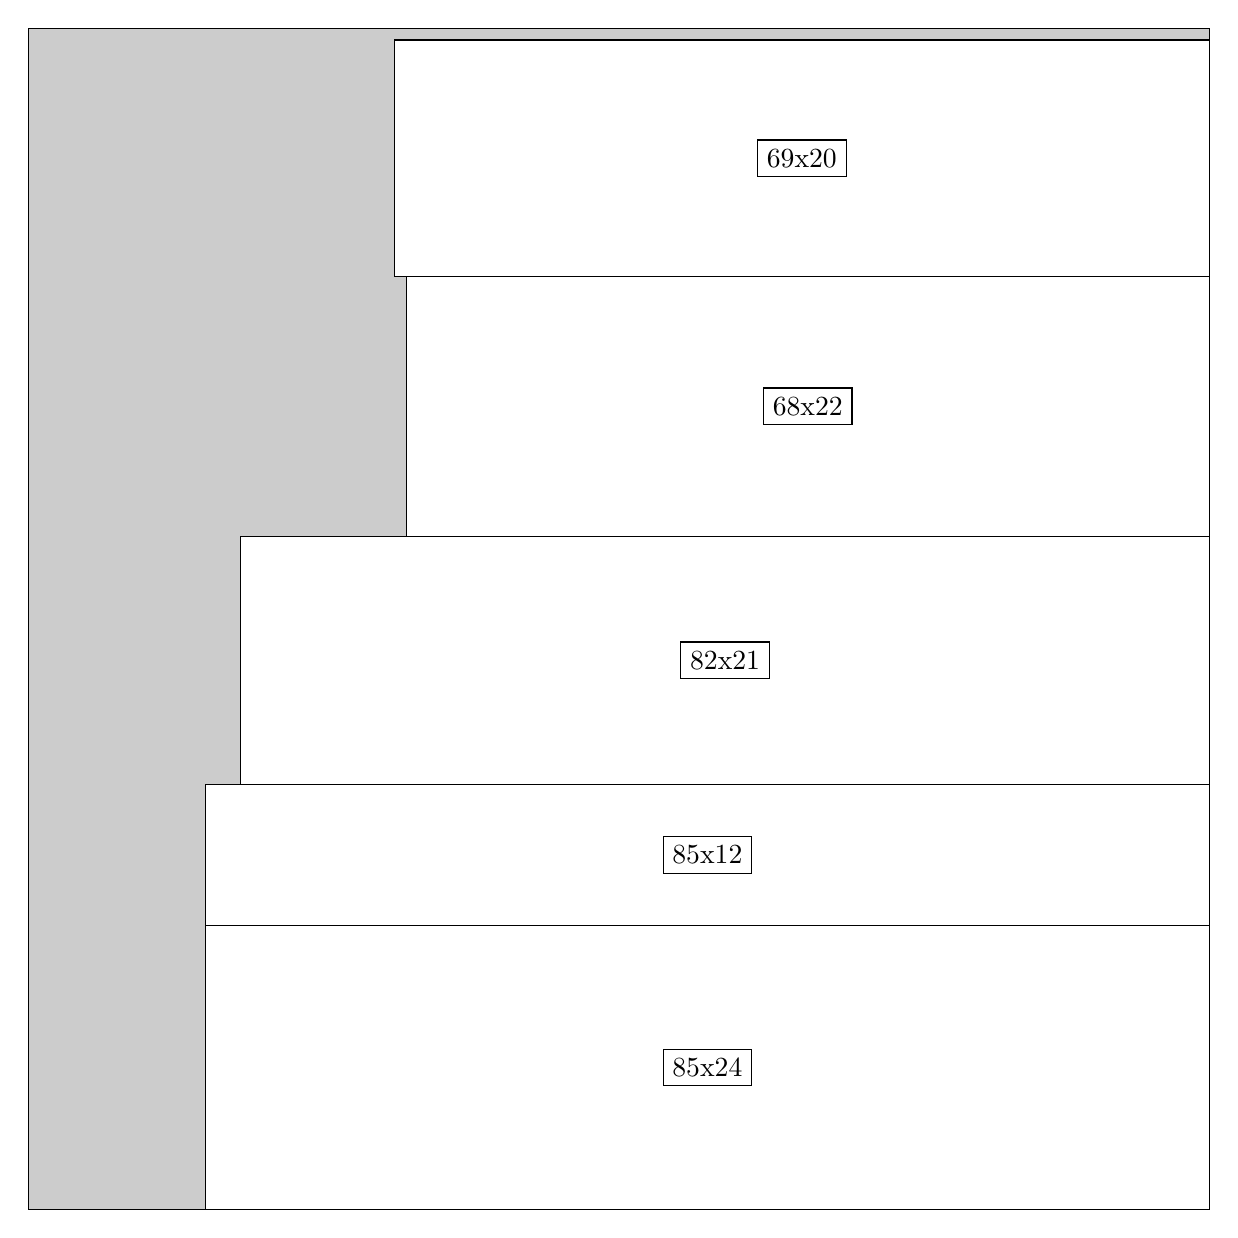
\begin{tikzpicture}[shorten >=1pt,scale=1.0,every node/.style={scale=1.0},->]
\tikzstyle{vertex}=[circle,fill=black!25,minimum size=14pt,inner sep=0pt]
\filldraw[fill=gray!40!white, draw=black] (0,0) rectangle (15.0,15.0);
\foreach \name/\x/\y/\w/\h in {85x24/2.25/0.0/12.75/3.5999999999999996,85x12/2.25/3.5999999999999996/12.75/1.7999999999999998,82x21/2.6999999999999997/5.3999999999999995/12.299999999999999/3.15,68x22/4.8/8.549999999999999/10.2/3.3,69x20/4.6499999999999995/11.85/10.35/3.0}
\filldraw[fill=white!40!white, draw=black] (\x,\y) rectangle node[draw] (\name) {\name} ++(\w,\h);
\end{tikzpicture}


w =85 , h =24 , x =15 , y =0 , v =2040
\par
w =85 , h =12 , x =15 , y =24 , v =1020
\par
w =82 , h =21 , x =18 , y =36 , v =1722
\par
w =68 , h =22 , x =32 , y =57 , v =1496
\par
w =69 , h =20 , x =31 , y =79 , v =1380
\par
\newpage


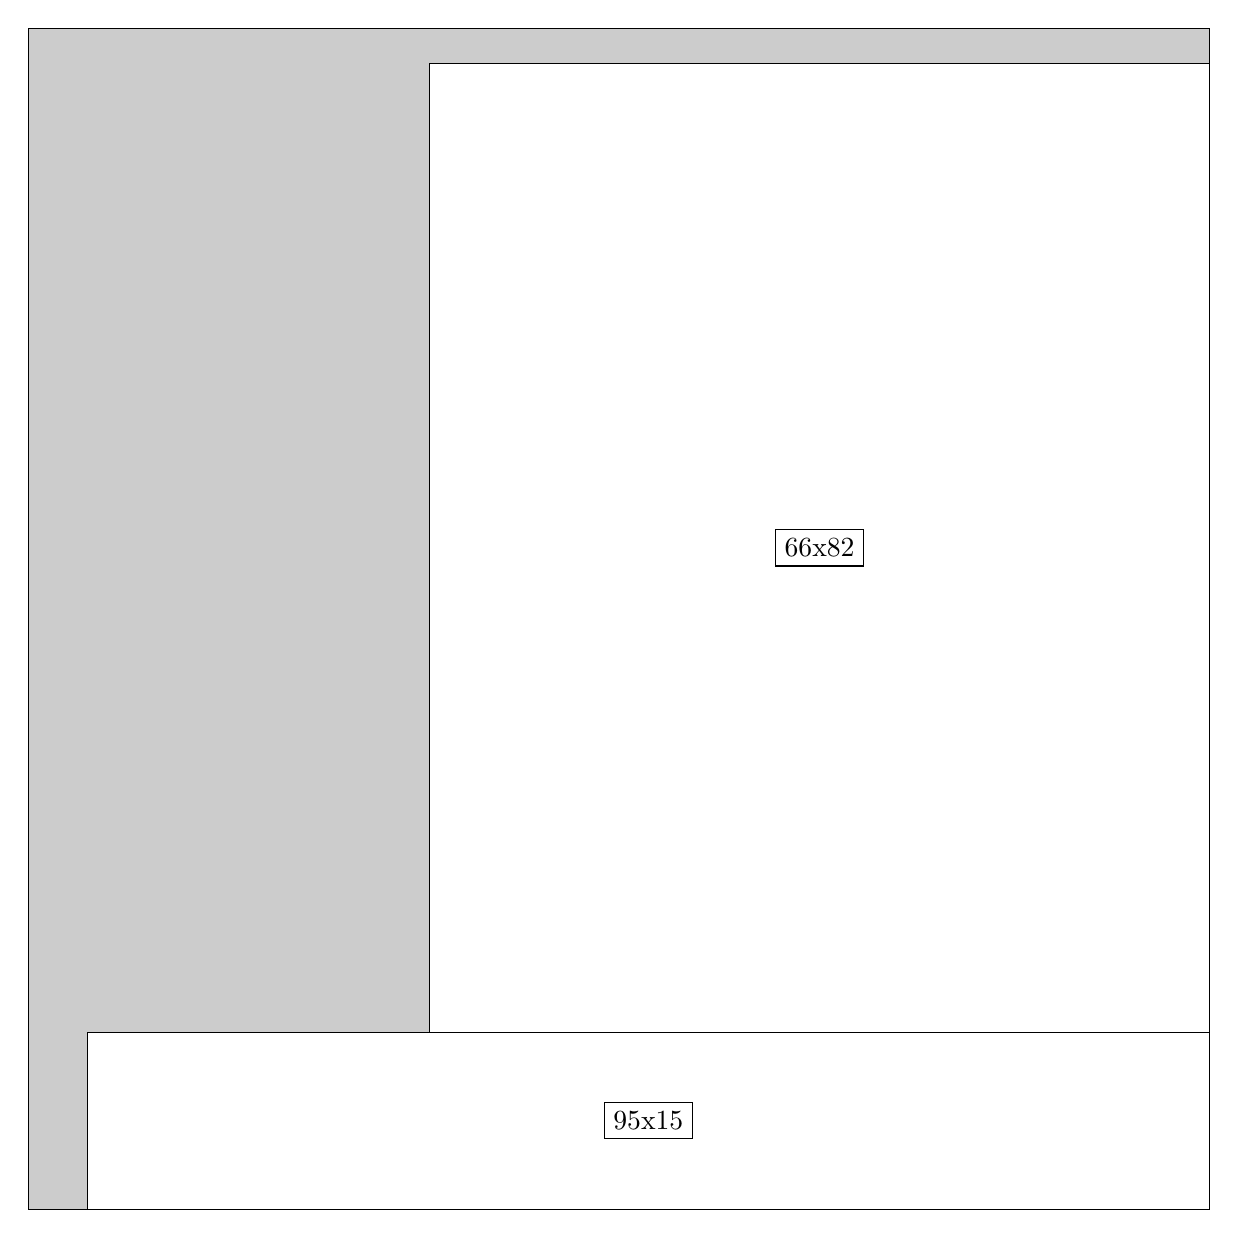
\begin{tikzpicture}[shorten >=1pt,scale=1.0,every node/.style={scale=1.0},->]
\tikzstyle{vertex}=[circle,fill=black!25,minimum size=14pt,inner sep=0pt]
\filldraw[fill=gray!40!white, draw=black] (0,0) rectangle (15.0,15.0);
\foreach \name/\x/\y/\w/\h in {95x15/0.75/0.0/14.25/2.25,66x82/5.1/2.25/9.9/12.299999999999999}
\filldraw[fill=white!40!white, draw=black] (\x,\y) rectangle node[draw] (\name) {\name} ++(\w,\h);
\end{tikzpicture}


w =95 , h =15 , x =5 , y =0 , v =1425
\par
w =66 , h =82 , x =34 , y =15 , v =5412
\par
\newpage


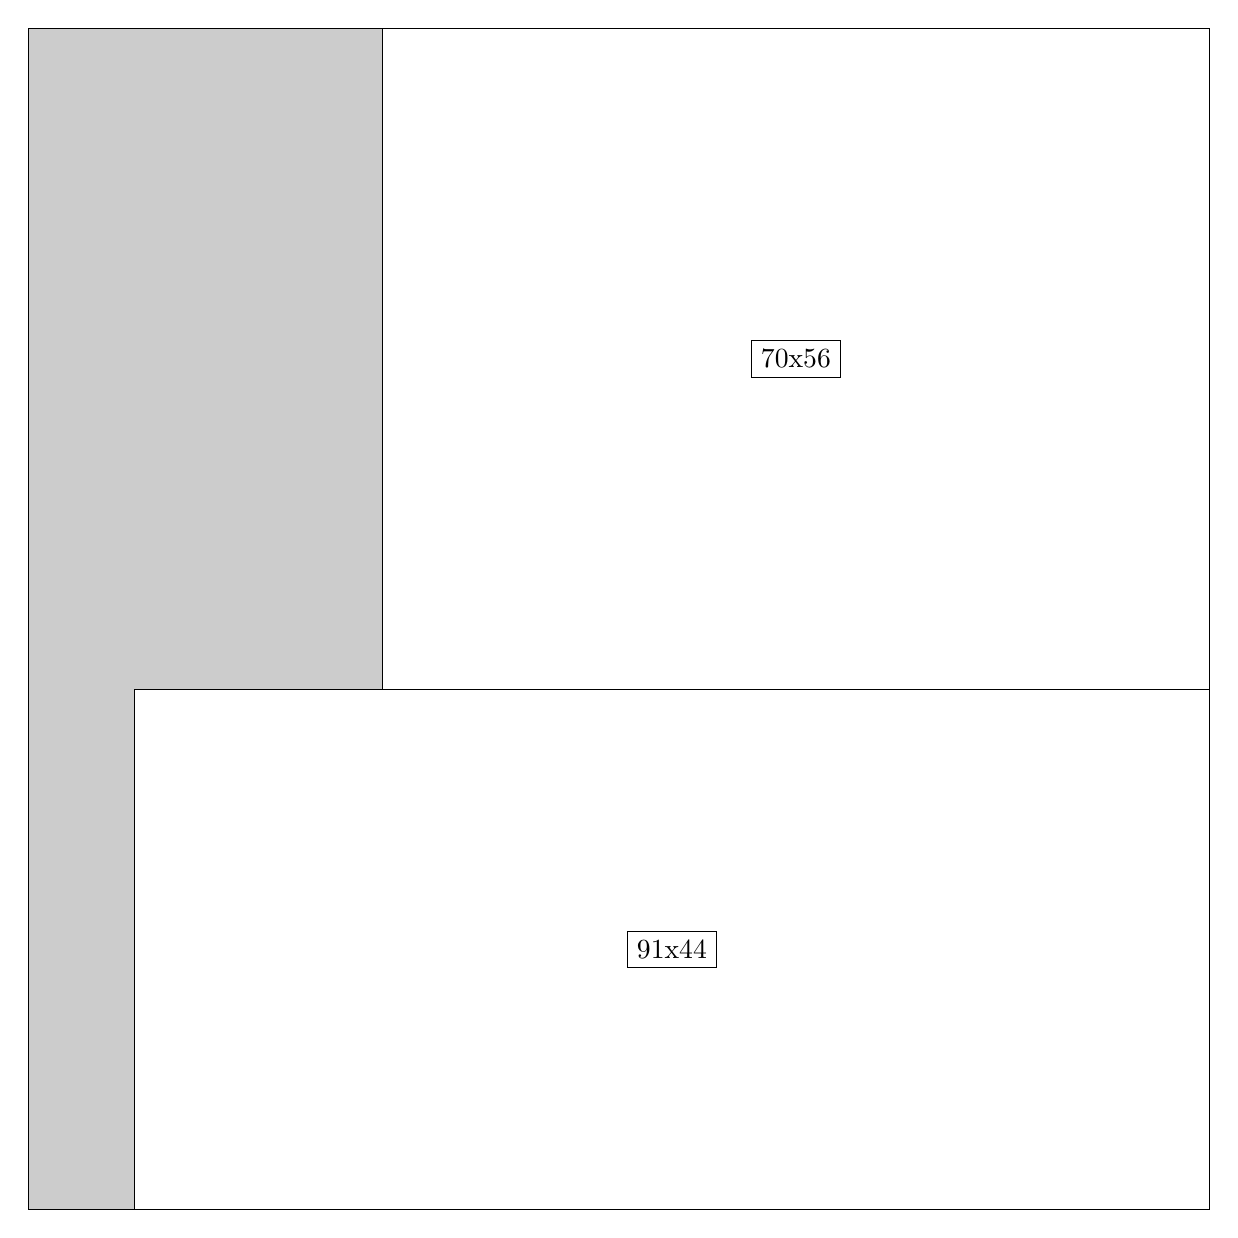
\begin{tikzpicture}[shorten >=1pt,scale=1.0,every node/.style={scale=1.0},->]
\tikzstyle{vertex}=[circle,fill=black!25,minimum size=14pt,inner sep=0pt]
\filldraw[fill=gray!40!white, draw=black] (0,0) rectangle (15.0,15.0);
\foreach \name/\x/\y/\w/\h in {91x44/1.3499999999999999/0.0/13.65/6.6,70x56/4.5/6.6/10.5/8.4}
\filldraw[fill=white!40!white, draw=black] (\x,\y) rectangle node[draw] (\name) {\name} ++(\w,\h);
\end{tikzpicture}


w =91 , h =44 , x =9 , y =0 , v =4004
\par
w =70 , h =56 , x =30 , y =44 , v =3920
\par
\newpage


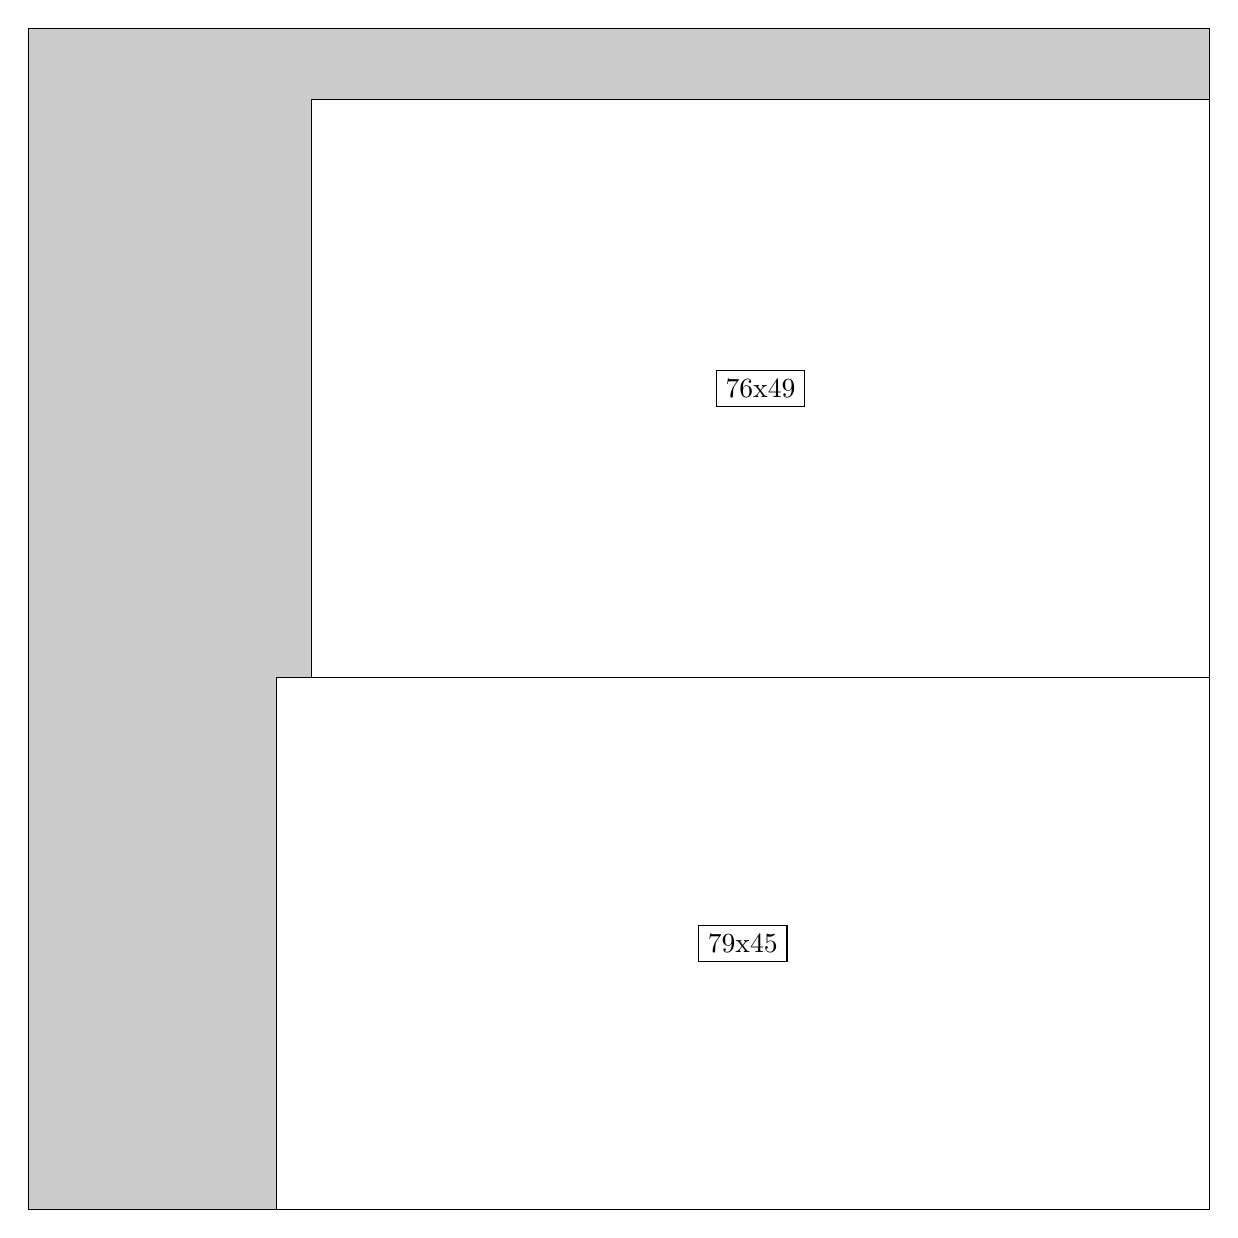
\begin{tikzpicture}[shorten >=1pt,scale=1.0,every node/.style={scale=1.0},->]
\tikzstyle{vertex}=[circle,fill=black!25,minimum size=14pt,inner sep=0pt]
\filldraw[fill=gray!40!white, draw=black] (0,0) rectangle (15.0,15.0);
\foreach \name/\x/\y/\w/\h in {79x45/3.15/0.0/11.85/6.75,76x49/3.5999999999999996/6.75/11.4/7.35}
\filldraw[fill=white!40!white, draw=black] (\x,\y) rectangle node[draw] (\name) {\name} ++(\w,\h);
\end{tikzpicture}


w =79 , h =45 , x =21 , y =0 , v =3555
\par
w =76 , h =49 , x =24 , y =45 , v =3724
\par
\newpage


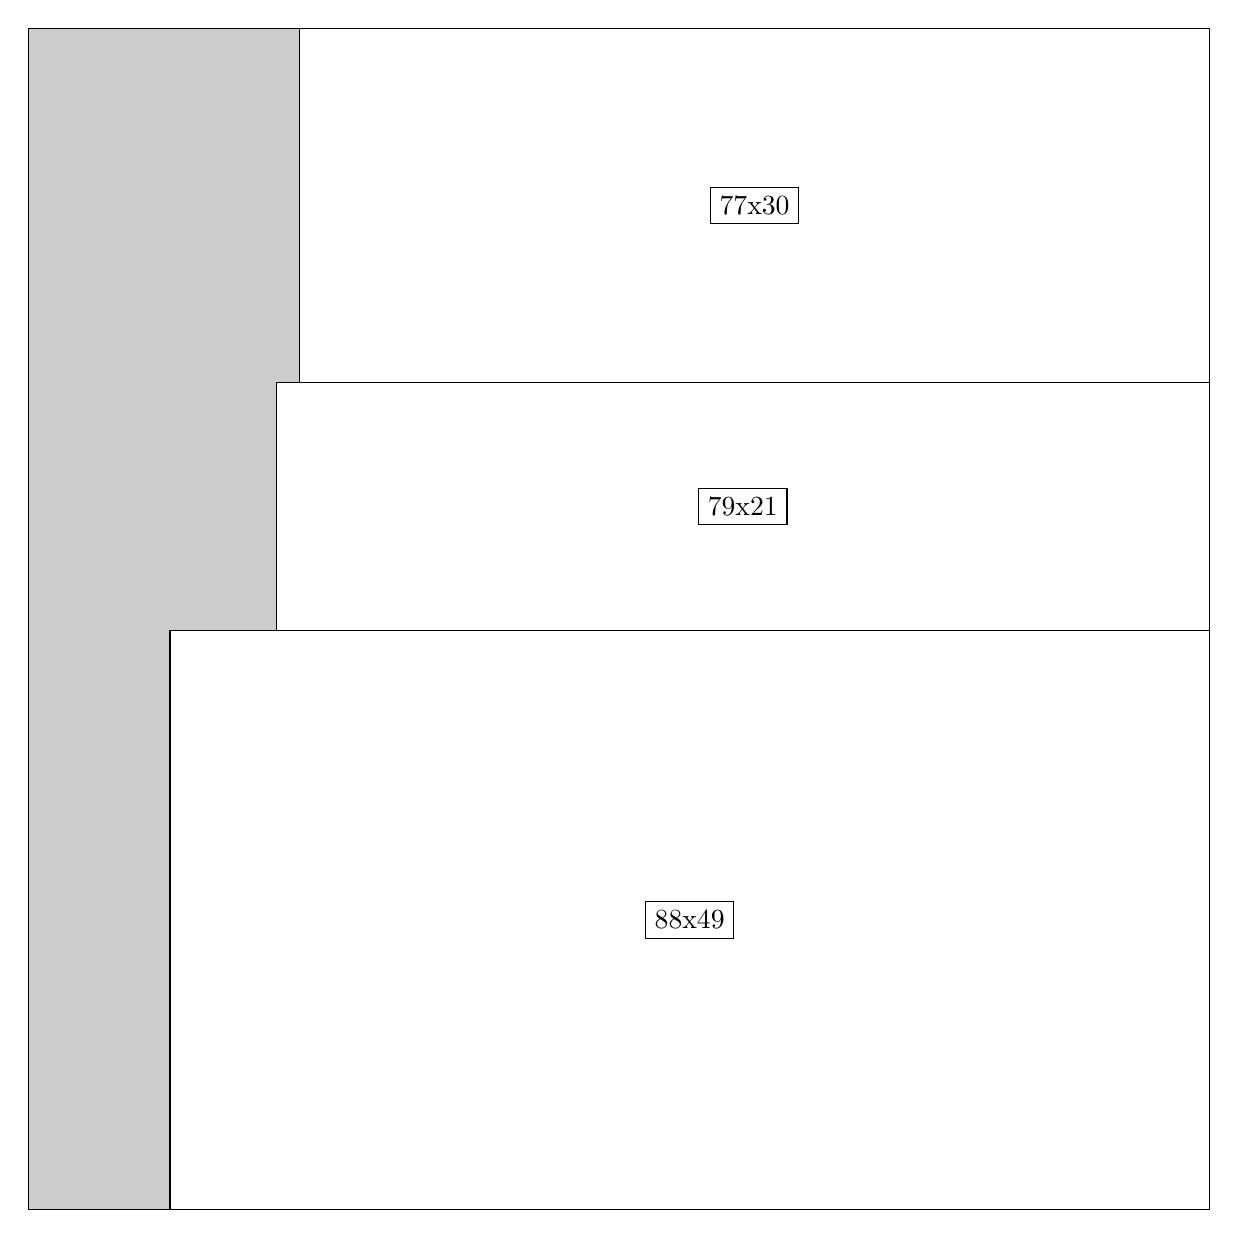
\begin{tikzpicture}[shorten >=1pt,scale=1.0,every node/.style={scale=1.0},->]
\tikzstyle{vertex}=[circle,fill=black!25,minimum size=14pt,inner sep=0pt]
\filldraw[fill=gray!40!white, draw=black] (0,0) rectangle (15.0,15.0);
\foreach \name/\x/\y/\w/\h in {88x49/1.7999999999999998/0.0/13.2/7.35,79x21/3.15/7.35/11.85/3.15,77x30/3.4499999999999997/10.5/11.549999999999999/4.5}
\filldraw[fill=white!40!white, draw=black] (\x,\y) rectangle node[draw] (\name) {\name} ++(\w,\h);
\end{tikzpicture}


w =88 , h =49 , x =12 , y =0 , v =4312
\par
w =79 , h =21 , x =21 , y =49 , v =1659
\par
w =77 , h =30 , x =23 , y =70 , v =2310
\par
\newpage


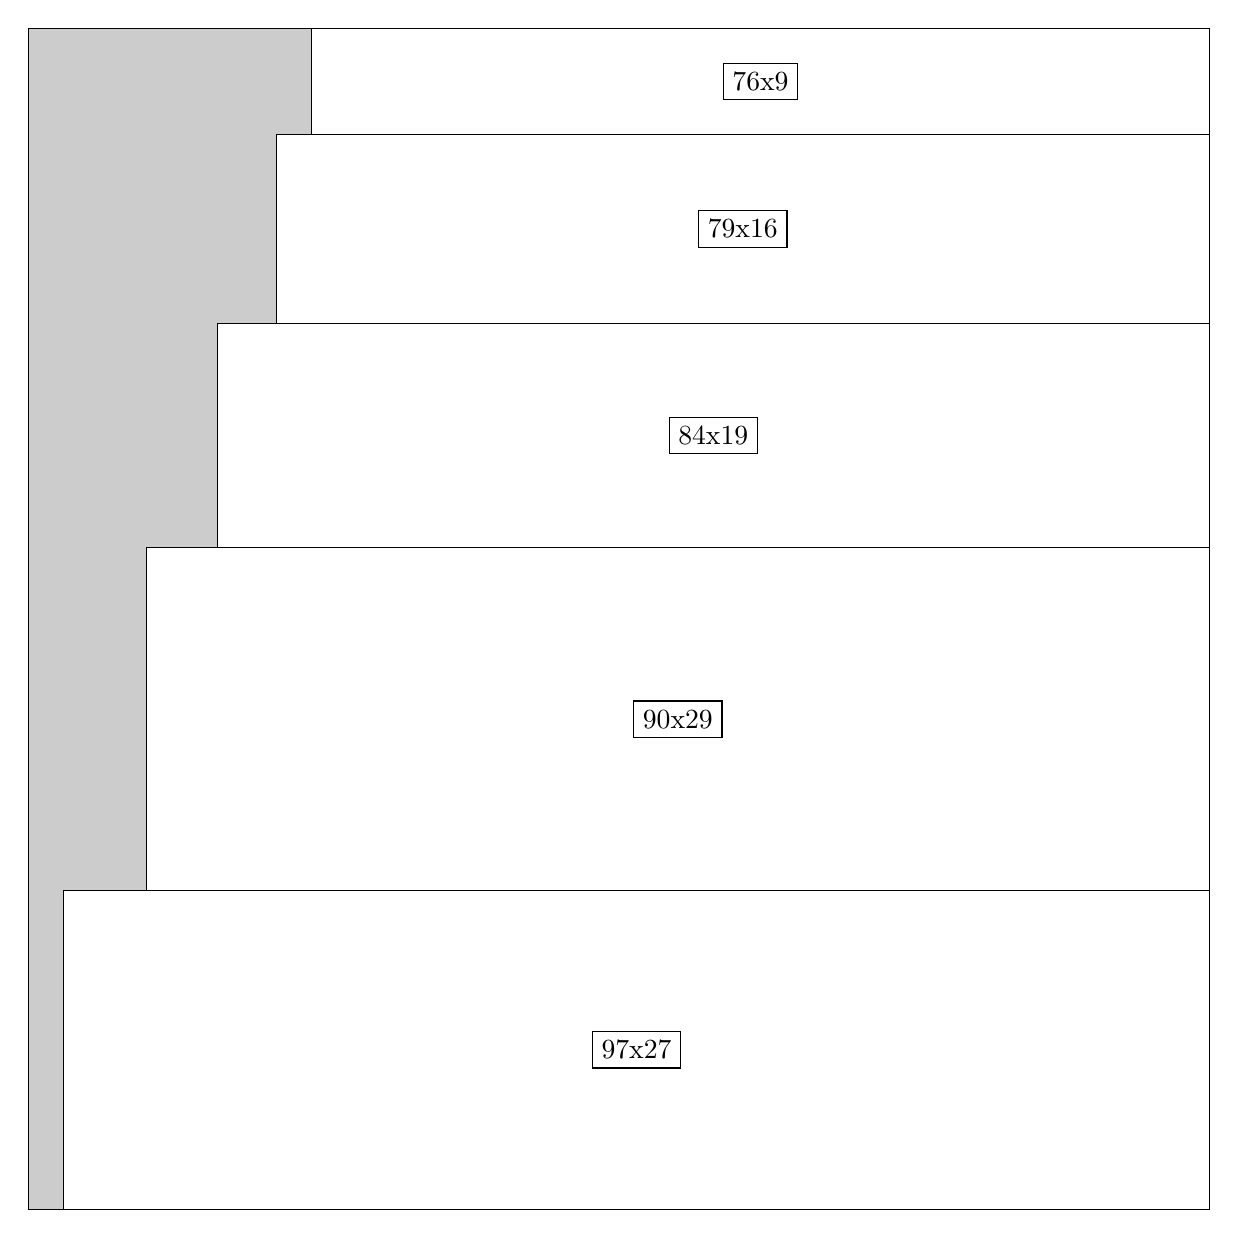
\begin{tikzpicture}[shorten >=1pt,scale=1.0,every node/.style={scale=1.0},->]
\tikzstyle{vertex}=[circle,fill=black!25,minimum size=14pt,inner sep=0pt]
\filldraw[fill=gray!40!white, draw=black] (0,0) rectangle (15.0,15.0);
\foreach \name/\x/\y/\w/\h in {97x27/0.44999999999999996/0.0/14.549999999999999/4.05,90x29/1.5/4.05/13.5/4.35,84x19/2.4/8.4/12.6/2.85,79x16/3.15/11.25/11.85/2.4,76x9/3.5999999999999996/13.65/11.4/1.3499999999999999}
\filldraw[fill=white!40!white, draw=black] (\x,\y) rectangle node[draw] (\name) {\name} ++(\w,\h);
\end{tikzpicture}


w =97 , h =27 , x =3 , y =0 , v =2619
\par
w =90 , h =29 , x =10 , y =27 , v =2610
\par
w =84 , h =19 , x =16 , y =56 , v =1596
\par
w =79 , h =16 , x =21 , y =75 , v =1264
\par
w =76 , h =9 , x =24 , y =91 , v =684
\par
\newpage


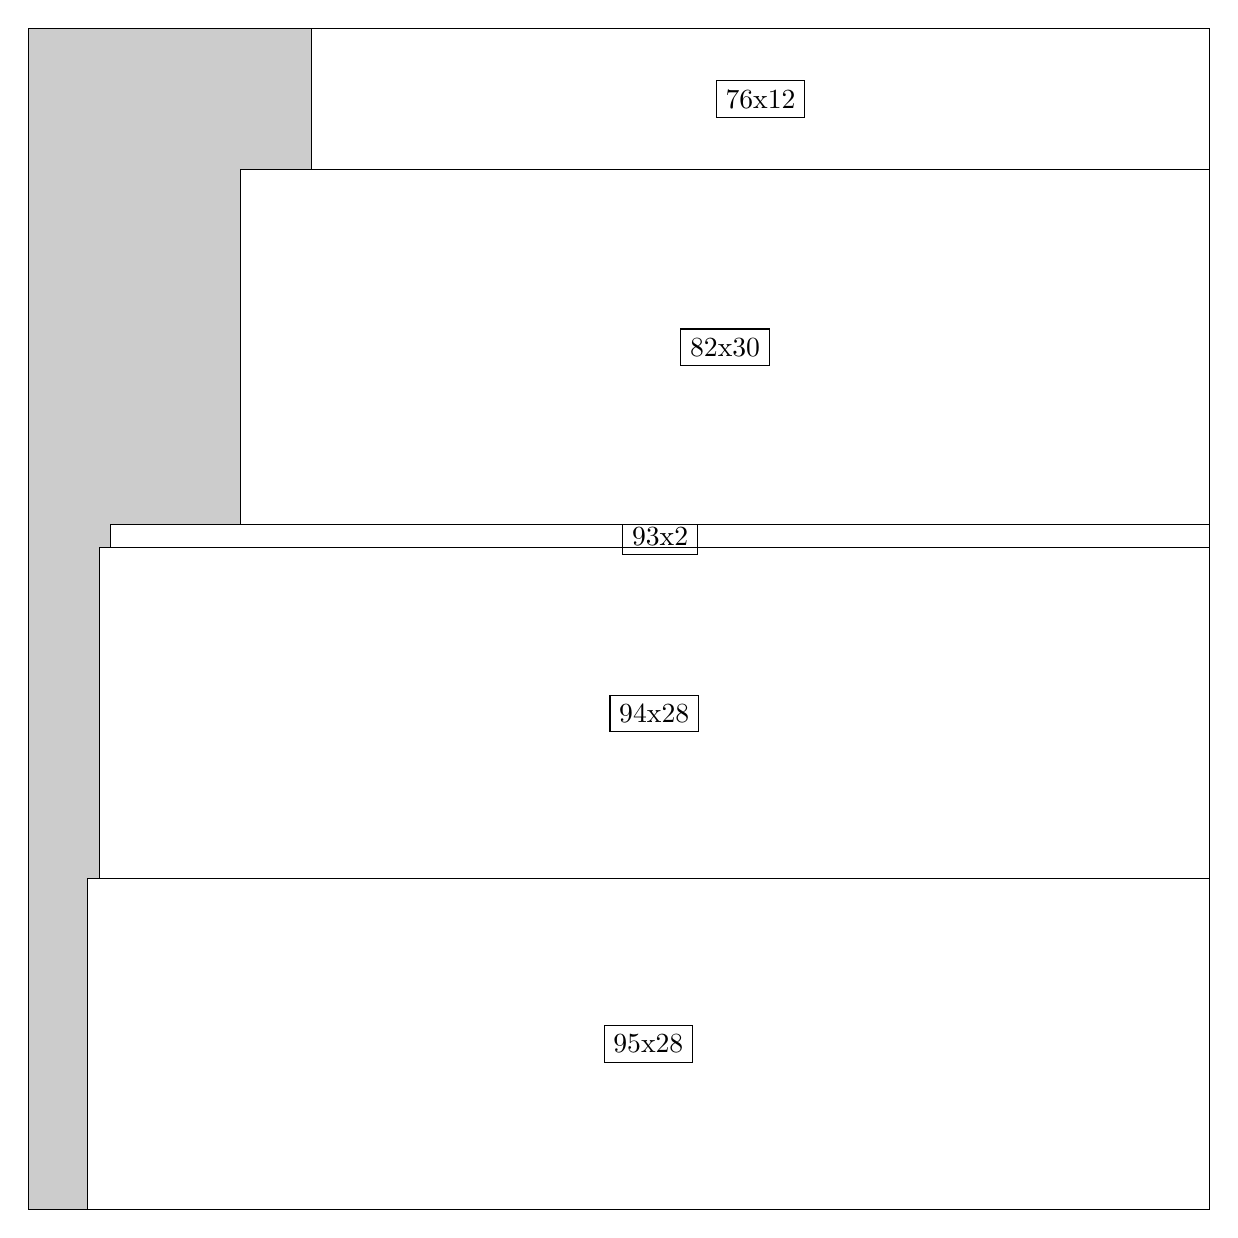
\begin{tikzpicture}[shorten >=1pt,scale=1.0,every node/.style={scale=1.0},->]
\tikzstyle{vertex}=[circle,fill=black!25,minimum size=14pt,inner sep=0pt]
\filldraw[fill=gray!40!white, draw=black] (0,0) rectangle (15.0,15.0);
\foreach \name/\x/\y/\w/\h in {95x28/0.75/0.0/14.25/4.2,94x28/0.8999999999999999/4.2/14.1/4.2,93x2/1.05/8.4/13.95/0.3,82x30/2.6999999999999997/8.7/12.299999999999999/4.5,76x12/3.5999999999999996/13.2/11.4/1.7999999999999998}
\filldraw[fill=white!40!white, draw=black] (\x,\y) rectangle node[draw] (\name) {\name} ++(\w,\h);
\end{tikzpicture}


w =95 , h =28 , x =5 , y =0 , v =2660
\par
w =94 , h =28 , x =6 , y =28 , v =2632
\par
w =93 , h =2 , x =7 , y =56 , v =186
\par
w =82 , h =30 , x =18 , y =58 , v =2460
\par
w =76 , h =12 , x =24 , y =88 , v =912
\par
\newpage


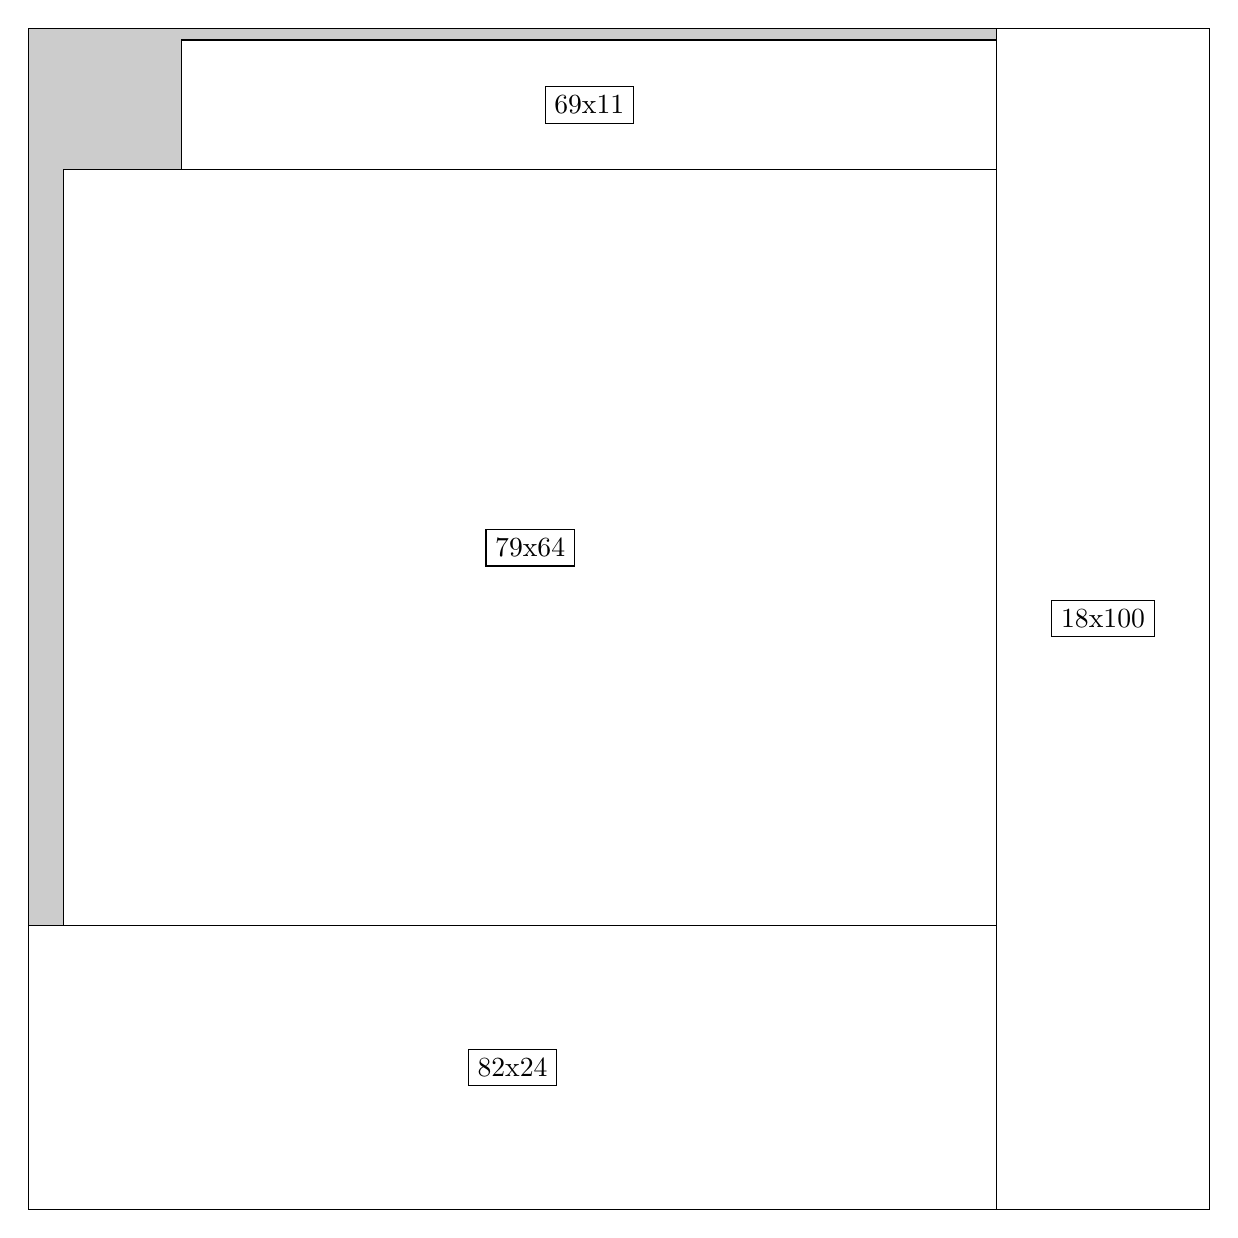
\begin{tikzpicture}[shorten >=1pt,scale=1.0,every node/.style={scale=1.0},->]
\tikzstyle{vertex}=[circle,fill=black!25,minimum size=14pt,inner sep=0pt]
\filldraw[fill=gray!40!white, draw=black] (0,0) rectangle (15.0,15.0);
\foreach \name/\x/\y/\w/\h in {18x100/12.299999999999999/0.0/2.6999999999999997/15.0,82x24/0.0/0.0/12.299999999999999/3.5999999999999996,79x64/0.44999999999999996/3.5999999999999996/11.85/9.6,69x11/1.95/13.2/10.35/1.65}
\filldraw[fill=white!40!white, draw=black] (\x,\y) rectangle node[draw] (\name) {\name} ++(\w,\h);
\end{tikzpicture}


w =18 , h =100 , x =82 , y =0 , v =1800
\par
w =82 , h =24 , x =0 , y =0 , v =1968
\par
w =79 , h =64 , x =3 , y =24 , v =5056
\par
w =69 , h =11 , x =13 , y =88 , v =759
\par
\newpage


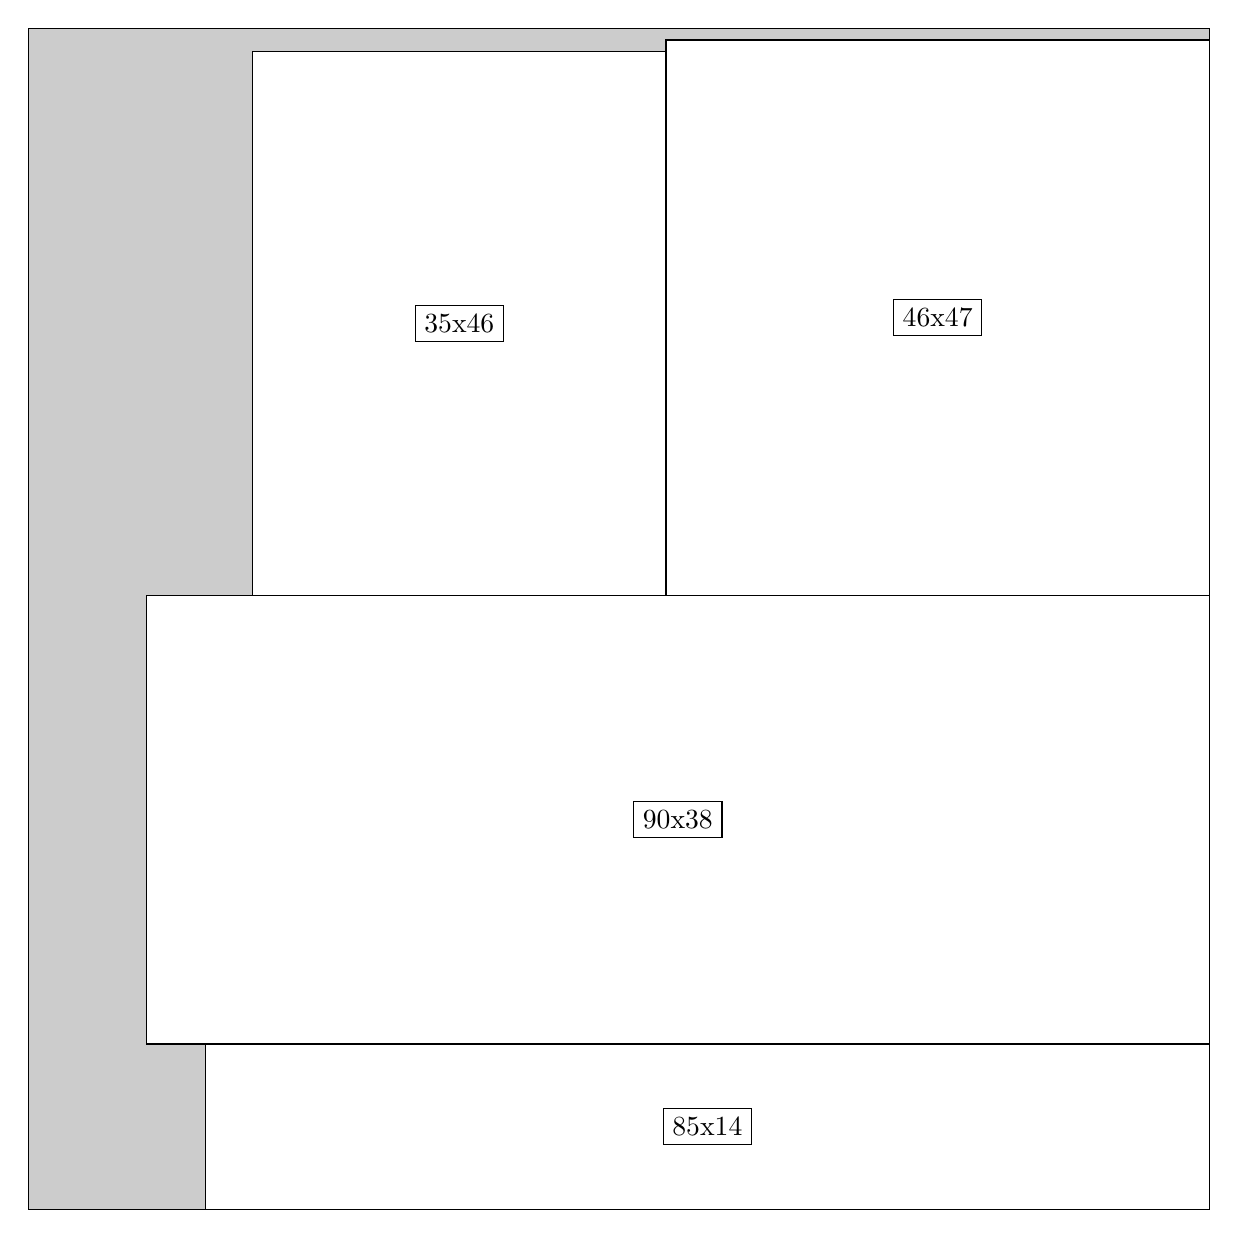
\begin{tikzpicture}[shorten >=1pt,scale=1.0,every node/.style={scale=1.0},->]
\tikzstyle{vertex}=[circle,fill=black!25,minimum size=14pt,inner sep=0pt]
\filldraw[fill=gray!40!white, draw=black] (0,0) rectangle (15.0,15.0);
\foreach \name/\x/\y/\w/\h in {85x14/2.25/0.0/12.75/2.1,90x38/1.5/2.1/13.5/5.7,46x47/8.1/7.8/6.8999999999999995/7.05,35x46/2.85/7.8/5.25/6.8999999999999995}
\filldraw[fill=white!40!white, draw=black] (\x,\y) rectangle node[draw] (\name) {\name} ++(\w,\h);
\end{tikzpicture}


w =85 , h =14 , x =15 , y =0 , v =1190
\par
w =90 , h =38 , x =10 , y =14 , v =3420
\par
w =46 , h =47 , x =54 , y =52 , v =2162
\par
w =35 , h =46 , x =19 , y =52 , v =1610
\par
\newpage


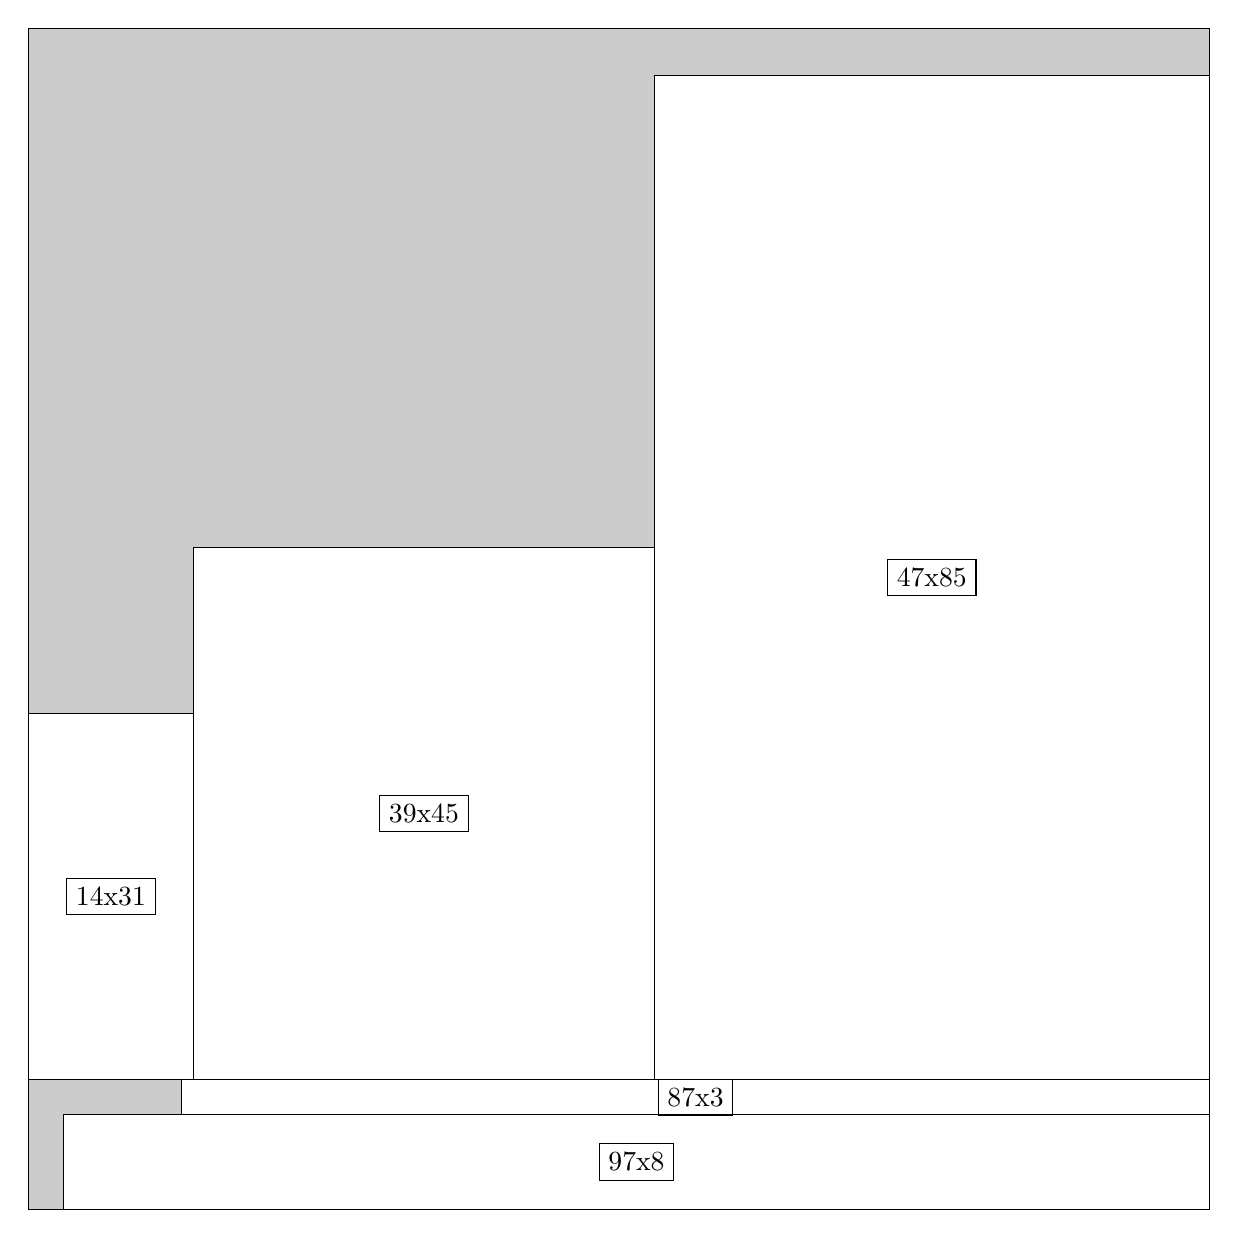
\begin{tikzpicture}[shorten >=1pt,scale=1.0,every node/.style={scale=1.0},->]
\tikzstyle{vertex}=[circle,fill=black!25,minimum size=14pt,inner sep=0pt]
\filldraw[fill=gray!40!white, draw=black] (0,0) rectangle (15.0,15.0);
\foreach \name/\x/\y/\w/\h in {97x8/0.44999999999999996/0.0/14.549999999999999/1.2,87x3/1.95/1.2/13.049999999999999/0.44999999999999996,47x85/7.949999999999999/1.65/7.05/12.75,39x45/2.1/1.65/5.85/6.75,14x31/0.0/1.65/2.1/4.6499999999999995}
\filldraw[fill=white!40!white, draw=black] (\x,\y) rectangle node[draw] (\name) {\name} ++(\w,\h);
\end{tikzpicture}


w =97 , h =8 , x =3 , y =0 , v =776
\par
w =87 , h =3 , x =13 , y =8 , v =261
\par
w =47 , h =85 , x =53 , y =11 , v =3995
\par
w =39 , h =45 , x =14 , y =11 , v =1755
\par
w =14 , h =31 , x =0 , y =11 , v =434
\par
\newpage


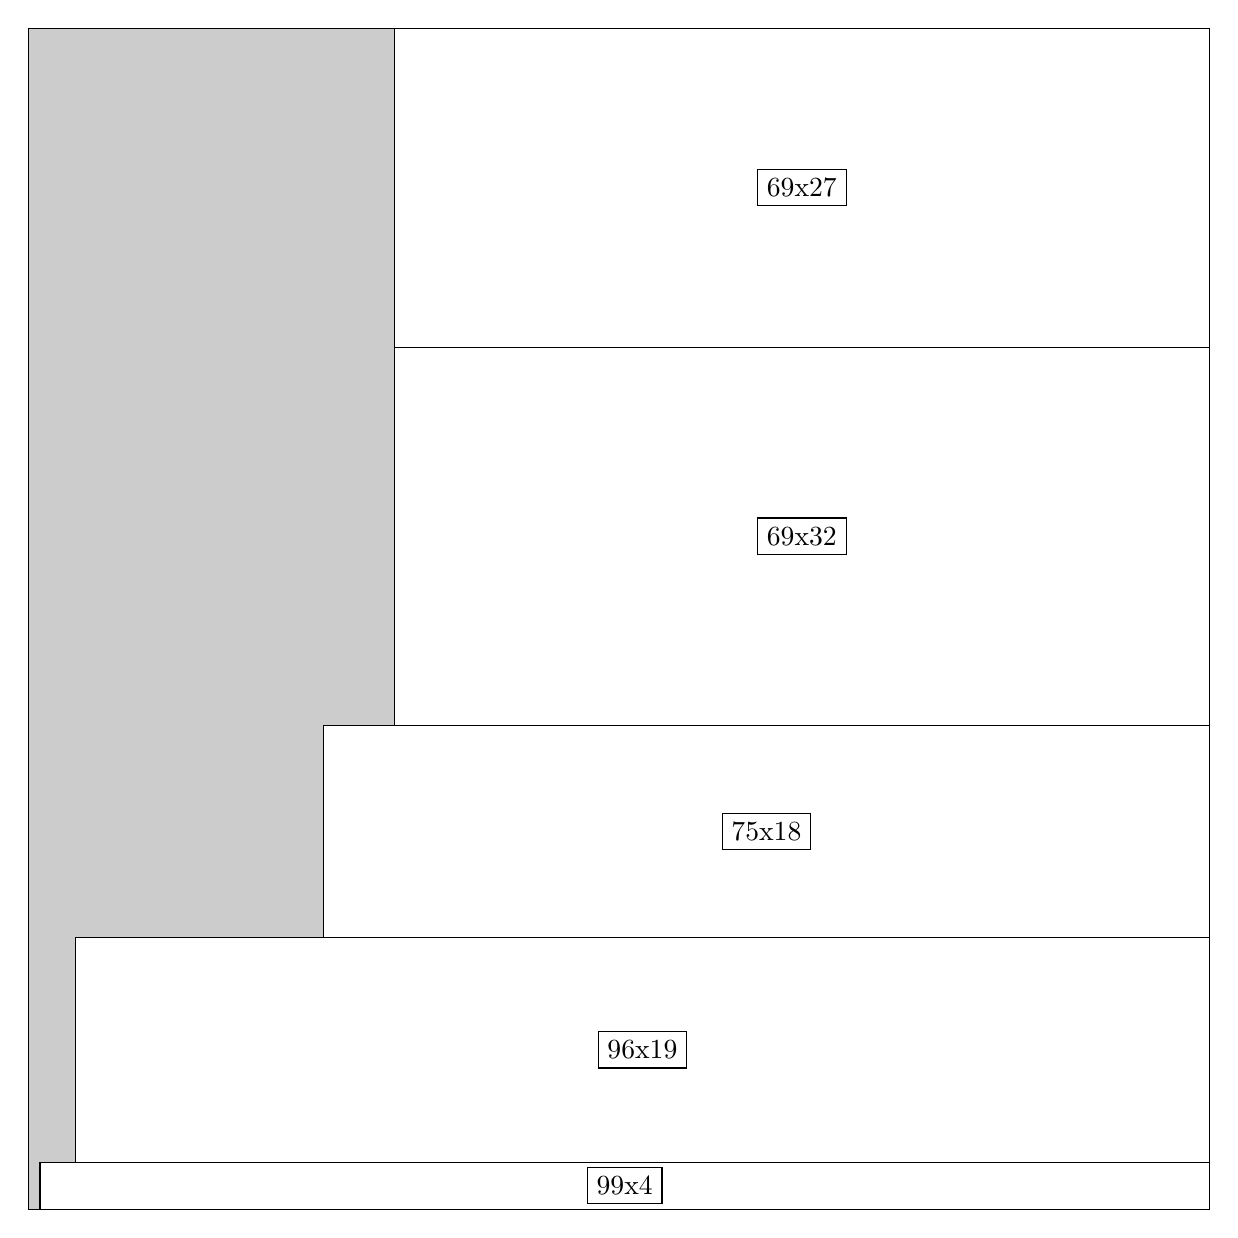
\begin{tikzpicture}[shorten >=1pt,scale=1.0,every node/.style={scale=1.0},->]
\tikzstyle{vertex}=[circle,fill=black!25,minimum size=14pt,inner sep=0pt]
\filldraw[fill=gray!40!white, draw=black] (0,0) rectangle (15.0,15.0);
\foreach \name/\x/\y/\w/\h in {99x4/0.15/0.0/14.85/0.6,96x19/0.6/0.6/14.399999999999999/2.85,75x18/3.75/3.4499999999999997/11.25/2.6999999999999997,69x32/4.6499999999999995/6.1499999999999995/10.35/4.8,69x27/4.6499999999999995/10.95/10.35/4.05}
\filldraw[fill=white!40!white, draw=black] (\x,\y) rectangle node[draw] (\name) {\name} ++(\w,\h);
\end{tikzpicture}


w =99 , h =4 , x =1 , y =0 , v =396
\par
w =96 , h =19 , x =4 , y =4 , v =1824
\par
w =75 , h =18 , x =25 , y =23 , v =1350
\par
w =69 , h =32 , x =31 , y =41 , v =2208
\par
w =69 , h =27 , x =31 , y =73 , v =1863
\par
\newpage


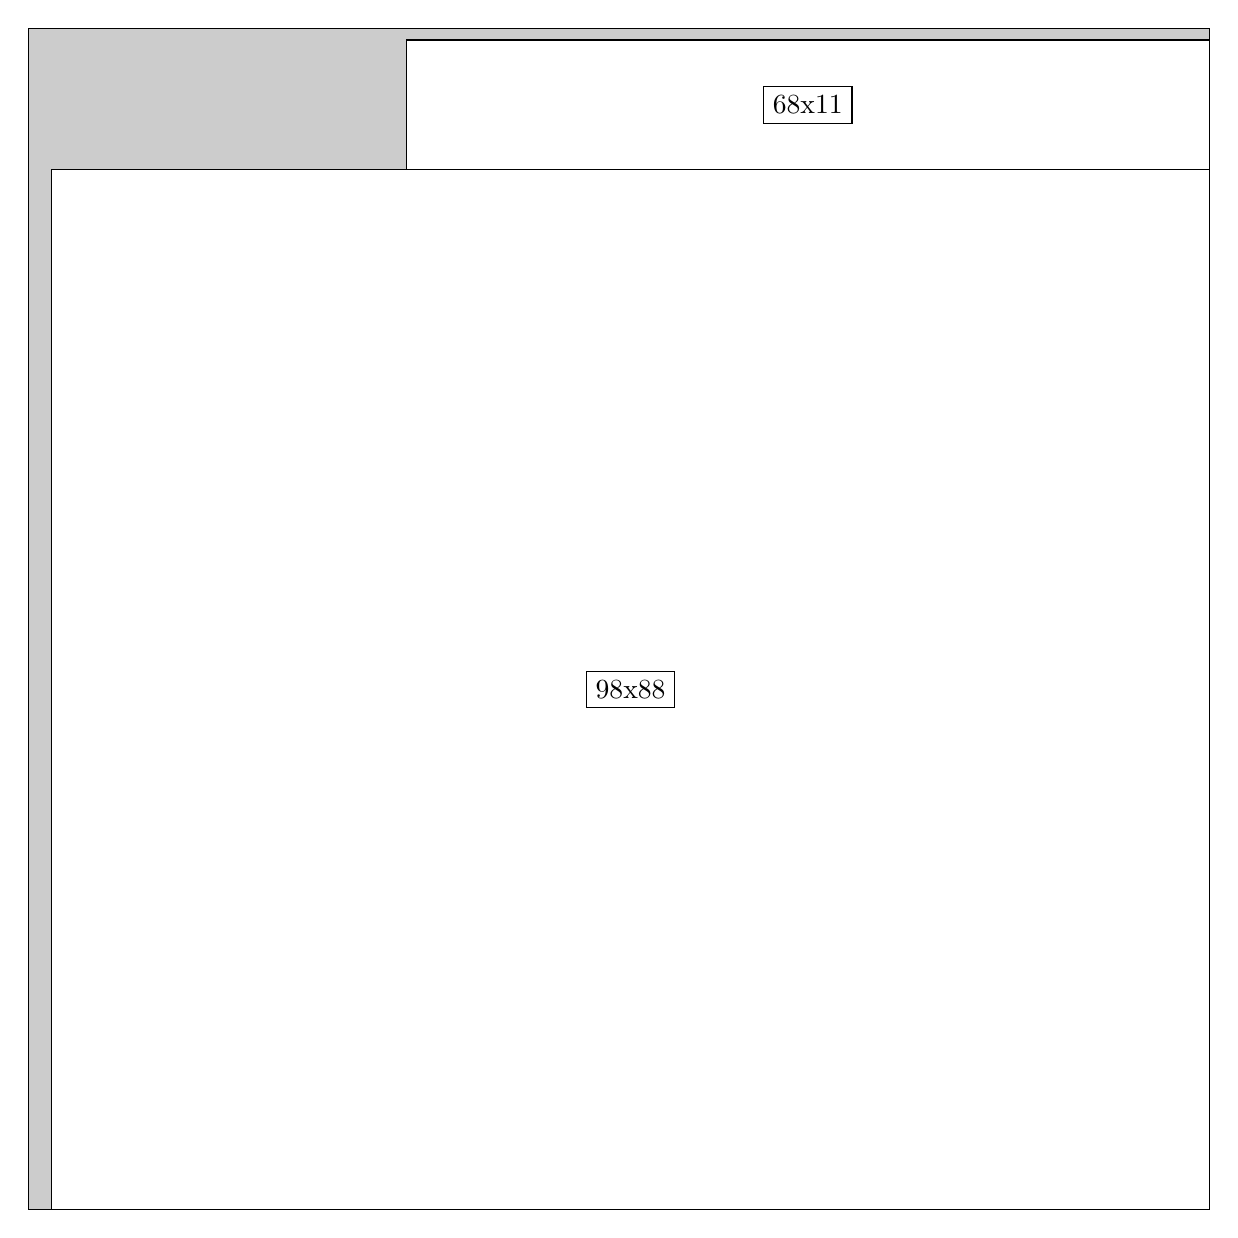
\begin{tikzpicture}[shorten >=1pt,scale=1.0,every node/.style={scale=1.0},->]
\tikzstyle{vertex}=[circle,fill=black!25,minimum size=14pt,inner sep=0pt]
\filldraw[fill=gray!40!white, draw=black] (0,0) rectangle (15.0,15.0);
\foreach \name/\x/\y/\w/\h in {98x88/0.3/0.0/14.7/13.2,68x11/4.8/13.2/10.2/1.65}
\filldraw[fill=white!40!white, draw=black] (\x,\y) rectangle node[draw] (\name) {\name} ++(\w,\h);
\end{tikzpicture}


w =98 , h =88 , x =2 , y =0 , v =8624
\par
w =68 , h =11 , x =32 , y =88 , v =748
\par
\newpage


\end{document}